% -*- coding: utf-8 -*-
\documentclass[UTF8,a4paper,10pt]{ctexart}
\usepackage[left=3.17cm, right=3.17cm, top=2.74cm, bottom=2.74cm]{geometry}
\usepackage{amsmath}
\usepackage{graphicx,subfig}
\usepackage{float}
\usepackage{cite}
\usepackage{caption}
\usepackage{enumerate}
\usepackage{booktabs} %表格
\usepackage{multirow}
\newcommand{\tabincell}[2]{\begin{tabular}{@{}#1@{}}#2\end{tabular}}  %表格强制换行
%-------------------------字体设置--------------
% \usepackage{times} 
\usepackage{ctex}
\setCJKmainfont[ItalicFont=Noto Sans CJK SC Bold, BoldFont=Noto Serif CJK SC Black]{Noto Serif CJK SC}


\newcommand{\yihao}{\fontsize{26pt}{36pt}\selectfont}           % 一号, 1.4 倍行距
\newcommand{\erhao}{\fontsize{22pt}{28pt}\selectfont}          % 二号, 1.25倍行距
\newcommand{\xiaoer}{\fontsize{18pt}{18pt}\selectfont}          % 小二, 单倍行距
\newcommand{\sanhao}{\fontsize{16pt}{24pt}\selectfont}  %三号字
\newcommand{\xiaosan}{\fontsize{15pt}{22pt}\selectfont}        % 小三, 1.5倍行距
\newcommand{\sihao}{\fontsize{14pt}{21pt}\selectfont}            % 四号, 1.5 倍行距
\newcommand{\banxiaosi}{\fontsize{13pt}{19.5pt}\selectfont}    % 半小四, 1.5倍行距
\newcommand{\xiaosi}{\fontsize{12pt}{18pt}\selectfont}            % 小四, 1.5倍行距
\newcommand{\dawuhao}{\fontsize{11pt}{11pt}\selectfont}       % 大五号, 单倍行距
\newcommand{\wuhao}{\fontsize{10.5pt}{15.75pt}\selectfont}    % 五号, 单倍行距
%-------------------------章节名----------------
\usepackage{ctexcap} 
\CTEXsetup[name={,、},number={ \chinese{section}}]{section}
\CTEXsetup[name={(,)},number={\chinese{subsection}}]{subsection}
\CTEXsetup[name={,.},number={\arabic{subsubsection}}]{subsubsection}
%-------------------------页眉页脚--------------
\usepackage{fancyhdr}
\pagestyle{fancy}
\lhead{\kaishu \leftmark}
% \chead{}
\rhead{\kaishu 计算机网络实验报告}
\lfoot{}
\cfoot{\thepage}
\rfoot{}
\renewcommand{\headrulewidth}{0.1pt}  
\renewcommand{\footrulewidth}{0pt}%去掉横线
\newcommand{\HRule}{\rule{\linewidth}{0.5mm}}%标题横线
\newcommand{\HRulegrossa}{\rule{\linewidth}{1.2mm}}
%-----------------------伪代码------------------
\usepackage{algorithm}  
\usepackage{algorithmicx}  
\usepackage{algpseudocode}  
\floatname{algorithm}{Algorithm}  
\renewcommand{\algorithmicrequire}{\textbf{Input:}}  
\renewcommand{\algorithmicensure}{\textbf{Output:}} 
\usepackage{lipsum}  
\makeatletter
\newenvironment{breakablealgorithm}
  {% \begin{breakablealgorithm}
  \begin{center}
     \refstepcounter{algorithm}% New algorithm
     \hrule height.8pt depth0pt \kern2pt% \@fs@pre for \@fs@ruled
     \renewcommand{\caption}[2][\relax]{% Make a new \caption
      {\raggedright\textbf{\ALG@name~\thealgorithm} ##2\par}%
      \ifx\relax##1\relax % #1 is \relax
         \addcontentsline{loa}{algorithm}{\protect\numberline{\thealgorithm}##2}%
      \else % #1 is not \relax
         \addcontentsline{loa}{algorithm}{\protect\numberline{\thealgorithm}##1}%
      \fi
      \kern2pt\hrule\kern2pt
     }
  }{% \end{breakablealgorithm}
     \kern2pt\hrule\relax% \@fs@post for \@fs@ruled
  \end{center}
  }
\makeatother
%------------------------代码-------------------
\usepackage{xcolor} 
\usepackage{listings} 
\usepackage{graphicx}
\lstset{ 
breaklines,%自动换行
basicstyle=\small,
escapeinside=``,
keywordstyle=\color{ blue!70} \bfseries,
commentstyle=\color{red!50!green!50!blue!50},% 
stringstyle=\ttfamily,% 
extendedchars=false,% 
linewidth=\textwidth,% 
numbers=left,% 
numberstyle=\tiny \color{blue!50},% 
frame=trbl% 
rulesepcolor= \color{ red!20!green!20!blue!20} 
}
%------------超链接----------
\usepackage[colorlinks,linkcolor=black,anchorcolor=blue]{hyperref}
%------------------------TODO-------------------
\usepackage{enumitem,amssymb}
\newlist{todolist}{itemize}{2}
\setlist[todolist]{label=$\square$}
% for check symbol 
\usepackage{pifont}
\newcommand{\cmark}{\ding{51}}%
\newcommand{\xmark}{\ding{55}}%
\newcommand{\done}{\rlap{$\square$}{\raisebox{2pt}{\large\hspace{1pt}\cmark}}\hspace{-2.5pt}}
\newcommand{\wontfix}{\rlap{$\square$}{\large\hspace{1pt}\xmark}}
%------------------------水印-------------------
\usepackage{tikz}
\usepackage{xcolor}
\usepackage{eso-pic}
\usepackage{verbatim}

\newcommand{\watermark}[3]{\AddToShipoutPictureBG{
\parbox[b][\paperheight]{\paperwidth}{
\vfill%
\centering%
\tikz[remember picture, overlay]%
  \node [rotate = #1, scale = #2] at (current page.center)%
    {\textcolor{gray!80!cyan!30!magenta!30}{#3}};
\vfill}}}
\lstset{
  basicstyle=\ttfamily\small, % 使用打字机字体并设置为小号
  numbers=left,
}
%———————————————————————————————————————————正文
%----------------------------------------------
\begin{document}
\begin{titlepage}
    \begin{center}
    
\includegraphics[width=0.8\textwidth]{NKU.png}\\[1cm]    
    \textsc{\Huge \kaishu{\textbf{南\ \ \ \ \ \ 开\ \ \ \ \ \ 大\ \ \ \ \ \ 学}} }\\[0.9cm]
    \textsc{\huge \kaishu{\textbf{网\ \ 络\ \ 空\ \ 间\ \ 安\ \ 全\ \ 学\ \ 院}}}\\[0.9cm]
    \textsc{\huge \kaishu{\textbf{计算机网络实验报告}}}\\[0.8cm]
    \HRule \\[0.9cm]
    { \LARGE \bfseries Lab3-3 选择确认实现可靠传输}\\[0.4cm]
    \HRule \\[2.0cm]
    \centering
    \textsc{\LARGE \kaishu{2113946\ \ \ 刘国民 }}\\[0.5cm]
    \textsc{\LARGE \kaishu{年级\ :\ 2021级}}\\[0.5cm]
    \textsc{\LARGE \kaishu{专业\ :\ 信息安全}}\\[0.5cm]
    \vfill
    {\Large \today}
    \end{center}
\end{titlepage}



\newpage
\tableofcontents
\setcounter{page}{1}

\vspace{1cm}

\section{实验内容}
本次实验依旧采用滑动窗口机制,并且在实验3-2的基础上,引入选择确认。即接收端在接收到失序的数据包时,会缓存下该数据包,并通知发送端已经缓存下该包,后续超时重发的时候不必重发该包。选择确认能够有效避免因为一个包的丢失,导致重发整个窗口数据包的问题发生。
\vspace{1cm}

\section{协议设计}
协议设计分为报文格式、差错检验、建立连接、数据传输和关闭连接五个部分。
\subsection{报文格式}
本次实验采用了两种不同的数据报格式,以发送端为例:
\begin{lstlisting}[frame=trbl,language={C++}]
struct Send_Datagram {
    bool ack, syn, fin, sack;
    uint16_t checksum;//16位校验和
    long long seqnum, acknum, sacknum;
    int DataLen;// DataLen<=MaxBufferSize
    char data[MaxBufferSize] = { 0 };
}SendData;

struct Receive_Datagram {
    bool ack, syn, fin, sack;
    uint16_t checksum;//16位校验和
    long long seqnum, acknum, sacknum;
    // 不需要数据缓冲区
}ReceiveData;
\end{lstlisting}\par
实验中定义了两种不同的数据报结构体,即发送数据报和接收数据报。考虑到实验情景为一端发送数据,另一端只负责接收数据并返回 ack,所以在接收数据报结构体中,本次实验去除了数据缓冲区,只包括 ack,syn,fin,sack 等必要的标志位、校验和以及序列号。注意标志位部分引入了 sack,下面我们给出标志位以及序列号的含义:
\begin{itemize}
    \item ack: 表示这是一个 ack 回复的数据包。接收端在回复确认报文时,将该标志位置为 true,发送端只在建立或者关闭连接时使用该标志位,实际传输时无需考虑。
    \item syn:建立连接时使用的标志位,表示一方请求与另一方建立连接。
    \item fin:关闭连接时使用的标志位,表示一方请求与另一方断开连接。
    \item sack:收到失序数据包时使用的标志位。
    \item seqnum=x:在传输过程中表示发送端发送了序号为 x 的数据包,这点与面向字节的 TCP 协议不同。和关闭连接中这个序号单独使用,后续相关部分会进行说明。
    \item acknum=x:在传输过程中表示接收端成功接收序号小于或等于 x 的数据包,这点也与面向字节的 TCP 协议不同。建立和关闭连接中这个序号单独使用,后续相关部分会进行说明。
    \item sacknum=x: 当 sack=true 的时候才使用的序号,表示收到了序号为 x 的失序数据包。
\end{itemize}\par
序列号方面实验仍然采用类似于 TCP 协议的非循环序列号,直接用一个 long long 类型保存即可。

\subsection{差错检验}
差错检验使用以下算法实现:
\begin{enumerate}
    \item 将数据报按16bit为一组进行分组,不足一组的用0补齐
    \item 将 checksum 字段置0
    \item 按位累加所有组的值,每次相加如果最高位有溢出则补到16位数的最低位上
    \item 将上述步骤的结果取反后填入 checksum 字段
\end{enumerate}\par
实验中用 RECEIVE\_CHECK和SEND\_CHECK 两个宏来标识是否取反,发送的时候需要取反,接受时则不用取反,接收时验证算出的校验和与数据包的校验和字段相加是否为 0xffff 即可。同时由于实验定义了两种不同的数据报文,所以在代码实现中利用函数重载的形式,分别实现了对两种报文的差错检验。

\subsection{建立连接}
依旧采用以下方式建立连接:
\begin{enumerate}
    \item 首先发送方发送一个空数据报给接收方(全为0),仅将 syn 标志位置为1,表示发送方请求建立连接。同时阻塞等待接收方的 syn+ack 包。
    \item 接收方持续阻塞等待发送方的 syn 包,如果成功接收到 syn 标志位为1的数据包,则将一个空包的 syn、ack 和 acknum 位置为1后发回,告诉发送方成功收到 seqnum 为0的 syn 包。
    \item 发送方成功收到 syn+ack 包后,发回一个 ack 包,同时设置 seqnum 和 acknum 为1,表示成功收到 seqnum 为0的 syn+ack 包,同时序列号自增1。至此连接建立完成,
\end{enumerate}\par
建立连接的具体流程基本与 TCP 三次握手一致,在这里双方的初始序列号 ISN 均取0。

\subsection{传输数据}
\begin{figure}[H]
    \centering
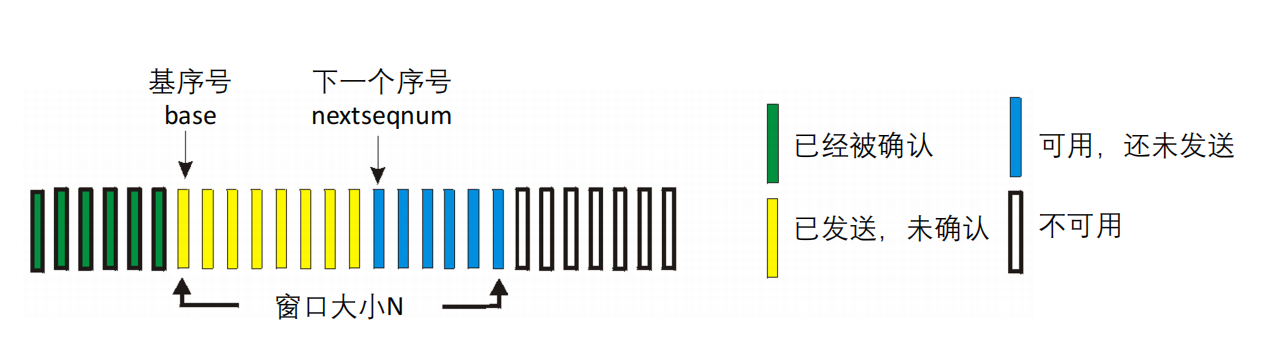
\includegraphics[width=0.6\textwidth]{img/滑动窗口.png}
    \caption{滑动窗口}
\end{figure}
传输数据部分的基本逻辑与上次实验相同,类似于 GBN 协议,只是在此基础上扩展了支持选择确认的功能,这里不再详细说明原有协议本身,重点阐述如何将选择确认补充到原有协议设计中。

\subsubsection{接收端逻辑}
在上次实验中,接收端维护一个期望序列号变量。如果收到的数据包序号等于期望序列号则写回文件,发回回复报文并让期望序列号加1;如果收到的数据包序号大于或者小于期望序列号,则发回一个 acknum 为期望序列号-1的回复报文,告诉发送端已经收到在此之前的,现在要期望序列号的数据包。本次实验中,我们对这个逻辑进行修改,即:
\begin{enumerate}
    \item 如果接收端收到的数据包大于期望值,则缓存下该数据包,不再发回 ack 包,而是将 sack 置为1,同时 sacknum 设置为收到数据包的数据号,即告诉发送端收到了序号为 sacknum 的失序包。
    \item 如果接收端收到的数据包等于期望值,则存下数据包,同时期望值+1。注意,这里还需要继续判断,如果期望值的数据包在之前已经缓存过了,则继续更新期望值,继续加1,直到期望序列号的数据包没有缓存过。最后再 acknum 期望值-1,表示在此之前(包含该序号)的数据包都已收到或缓存。
    \item 如果接收端收到的数据包小于期望值,与上次实验类似,直接丢弃即可。
\end{enumerate}\par

\subsubsection{发送端逻辑}
发送端的逻辑变化主要在于接收 ack  回复和重发窗口数据包的时候。在之前的实验中,发送端为 Base 数据包启动定时器,如果收到的 ack 包的回复序列号 acknum >= Base 则重置定时器,并且更新 Base 的值。本次实验由于新引入了 sack,所以逻辑也需要更改。即如果收到了 sack 包,则表示序号为 sacknum 的数据包已经被接收端成功缓存。后续涉及重发窗口的时候,遇到该序号的数据包直接跳过即可,不需要重发。注意收到 sack 的时候不能重置定时器,仍然需要为 Base 包的回复报文计时。

\subsubsection{情形分析}
基于设计的协议,我们分析丢失、错误等各种情形下该协议是怎么运转的,遇到问题后能否正确恢复。
\begin{enumerate}
    \item 发送数据包丢失/出错: 序号为 x 的数据包丢失后,之前的数据包都已成功收到 ack 的回复报文,则窗口右移到该包,此时 Base=x,开启定时器后,假设后续窗口中的所有数据包都成功抵达接收端。接收端收到后失序缓存下这些数据包,并发回 sack 报文,但发送端仍然未等到 Base 包的回复报文,最终超时重传窗口,而窗口中后续数据包都已成功抵达,发送端重发 Base 包即可,此时接收端成功收到后,由于该包填上了空缺,回复报文的 acknum 变为 Base+WindowSize。发送端收到该报文后则知道在此之前(包含该序号)的数据包都成功收到,直接更新 Base 包即可,继续传输。在这里我们考虑下更极端的情形,假如 sack 报文丢失或出错,那么发送端则不知道接收端已经成功缓存后续数据包,重发窗口时会再次发送这些数据包,根据协议设计,接收端仍然按照三种情况判断即可,不会影响传输;再假如填上空缺后接收端回复的 ack 报文丢失了怎么办?这里其实跟下面一种情况是一样的,直接看下面的逻辑即可。
    \item ack丢失/出错/提前超时:假设接收端收到了 seqnum=x 的数据包,此时发送一个 acknum=x 的回复报文给发送端,并且期望值+1,如果该包丢失、出错或者提前超时了,但接收端也收到了后续的数据包(x+1,x+2,...),之后的回复报文没有丢失、出错,则发送端收到的 acknum > Base,直接更新 Base,窗口右移即可;如果后续数据包丢失出错或者回复的 ack 丢失出错,则 Base 包超时,发送端重发窗口。这个过程中没有涉及选择确认和失序缓存,发送端发送后,接收端收到序号小于期望值的数据包,给出期望值-1的回复报文,则发送端可以直接调整 Base,继续正常传输。
\end{enumerate}

\subsection{关闭连接}
关闭连接也使用与TCP协议类似的流程,如下图所示:
\begin{figure}[H]
    \centering
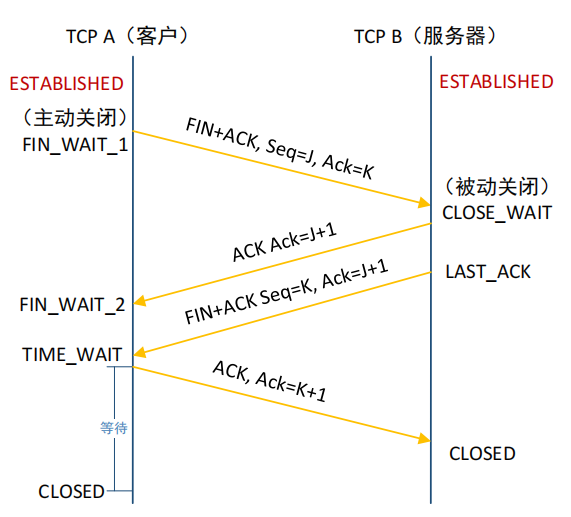
\includegraphics[width=0.6\textwidth]{img/关闭连接.png}
    \caption{关闭连接}
\end{figure}
如上图所示,但序列号J和K在此处跟三次握手类似,均取为0。

\section{代码实现}
代码实现部分主要分析传输数据和差错检验部分的代码,Socket 初始化、建立和关闭连接的代码与上次实验基本相同,不再赘述。建立连接时,我将发送数据报的总数放入了第一次握手 SYN 报文的空闲缓冲区,将文件名放入了第三次握手 ACK 报文的空闲缓冲区,一起发送给接收端。
\subsection{发送端}
与上次实验类似,发送端仍然使用三个线程,具体如下:
\begin{itemize}
\item 发送端用主线程 main 和两个创建的子线程 Resend 和 Timer 完成协议给出的功能和操作。
\item 主线程 main 负责发送数据包,即一旦窗口左边界右移,主线程负责发送新的数据包给接收端。
\item 子线程 Resend 负责持续检测是否“超时”,“超时”则重传,这里的“超时”指的是在指定时间内没有收到正确的 acknum (即 acknum >=Base)。
\item 子线程Timer负责为Base包开启定时器,一旦超时则通知线程Resend,这里的“通知”是通过全局变量的设置来实现,稍后会在具体的代码实现中看到。如果收到 sack,则记录sacknum的值,重传的时候跳过该包,这里的“记录”通过一个布尔数组来实现。 
\end{itemize}

首先给出差错检验函数:
\begin{lstlisting}[frame=trbl,language={C++}]
uint16_t Checksum(Send_Datagram d, int flag) {
    unsigned short* check = (unsigned short*)&d;//两字节为一组来处理
    int count = Send_DatagramLen / sizeof(short);// 一个数据报有 count 组
    d.checksum = 0;
    unsigned long sum = 0;
    while (count--) {
        sum += *check;
        check++;
        if (sum & 0xffff0000) {// 最高位有溢出
            sum = sum & 0xffff;
            sum++;
        }
    }
    if (flag == SEND_CHECK) {
        return (~sum) & 0xffff;//取反
    }
    else {
        return sum & 0xffff;
    }
}

// 利用函数重载
uint16_t Checksum(Receive_Datagram d, int flag) {
    unsigned short* check = (unsigned short*)&d;//两字节为一组来处理
    int count = Receive_DatagramLen / sizeof(short);// 一个数据报有 count 组
    d.checksum = 0;
    unsigned long sum = 0;
    while (count--) {
        sum += *check;
        check++;
        if (sum & 0xffff0000) {// 最高位有溢出
            sum = sum & 0xffff;
            sum++;
        }
    }
    if (flag == SEND_CHECK) {
        return (~sum) & 0xffff;//取反
    }
    else {
        return sum & 0xffff;
    }
}
\end{lstlisting}
代码基本按协议设计中给出的算法实现,两个函数逻辑相同,只是函数形参参中数据报类型不同,直接使用的函数重载,没有使用C++ 的模版特性。我们给出下列全局变量:
\begin{lstlisting}[frame=trbl,language={C++}]
// 多线程共享数据,写数据的时候用互斥锁
int Flag_Resend = 0;// 表示recvfrom的数据是否超时
int Flag_Timer = 0;// 表示是否需要启用定时器服务
int SeqNumber = 0;// 记录一共有多少个数据包,seqnum:0--SeqNumber-1
long long Base = 0;// 初始序列号从0开始
long long NextSeq = 0;

vector<Send_Datagram> v;//用来保存数据包序列
bool* flag_cache;// 指示某个包是否被缓存
\end{lstlisting}\par
从注释中可以看到,Flag\_Resend 用于表示收到的数据是否超时,只要子线程 Timer 发现超时了就将该标志位置为1,这时候子线程 Resend 就可以检测到,从而开始重发窗口中的数据包。Flag\_Timer 用于表示是否需要开启定时器,即主线程或者 
 Resend 线程发送 Base 包,或者窗口右移更新 Base 值的时候,就将该标志位置为1,Timer 线程就会开始启用定时器,持续接收可能的 ACK 回复。而 Base,NextSeq 和 SeqNumber 为全局变量,为三个线程共同使用。\par
我们用一个 bool 数组来指示某个包是否被缓存,bool[i]=true 则说明序列号为 i 的数据包被缓存。再用一个 vecotr 容器来保存所有要传输的数据包,在传输之前我们先把原始文件以4096字节为一组放入 vector 中,具体代码如下:
\begin{lstlisting}[frame=trbl,language={C++}]
// 移动文件指针到文件末尾
fseek(p, 0, SEEK_END);
long long FileLen = ftell(p);
fseek(p, 0, SEEK_SET);
long long temp = FileLen;
// 数据以4096字节为单位放入vector序列
while (temp>0) {
    SendData = { 0 };
    fread(SendData.data, MaxBufferSize, 1, p);
    SendData.DataLen = temp < MaxBufferSize ? temp : MaxBufferSize;
    SendData.seqnum = SeqNumber++;
    v.push_back(SendData);
    temp -= SendData.DataLen;
}
\end{lstlisting}\par
fread 将数据读取到发送数据包缓冲区中,将相关信息封装好后放入容器,之后涉及重传的时候,直接从容器中拿取数据包重发即可,对于窗口的滑动,直接增加 Base,NextSeq 等变量后通过vector随机访问即可,SeqNumber 用来记录一共有多少个数据包。接下来我们逐个分析三个线程的具体代码。
\begin{lstlisting}[frame=trbl,language={C++}]
while (true) {
    if (NextSeq == SeqNumber) {// 发送完毕
        break;
    }
    if (NextSeq < Base + WindowSize) {
        SendData = v[NextSeq];
        Send();
        if (NextSeq == Base) {// 第一个包
            lock_guard<mutex> lock(mtx);
            Flag_Timer = 1;
        }
        {
            lock_guard<mutex> lock(mtx);
            NextSeq++;
        }
        Sleep(100);;//每次发送睡眠100毫秒,避免短时间内发送大量数据包给接收方
    }
}
\end{lstlisting}\par
上述代码是 main 函数中发送数据的核心代码,整体逻辑是持续检测 NextSeq 是否小于 Base+WindowSize,即发送的数据包是否到达右边界,如果没到达就持续发送并增加 NextSeq 的值。如果发送的是 Bas e包则需要设置 Timer 标志位,通知子线程启动定时器。其中 v 即是上述提到的 vector 容器,需要注意在这个过程中,对多线程的共享数据(这里为 Flag\_Timer)进行写操作时,需要使用互斥锁以阻塞子线程进行操作,避免多线程同时进行写操作从而引发错误。每次发送后,使用 sleep 函数睡眠100毫秒,避免短时间发送大量数据包给接收方。如果 NextSeq 等于 SeqNumber,则代表窗口右边界已经到达容器末尾,此时主线程直接 break 退出循环即可。后续可能涉及到的重传由 Resend 完成。
\begin{lstlisting}[frame=trbl,language={C++}]
void Resend() {// 只要检测到Flag_Resend变为1就重发Base--(NextSeq-1)
    while (true) {
        if (Flag_Resend == 1) {
            BackCounter++;
            int curr = 0;
            for (int i = Base; i <= NextSeq - 1; i++) {
                // 首先根据失序数据包序列判断是否需要重发
                if (flag_cache[i]) continue;
                SendData = v[i];
                Send();
                if (i == Base) {//Base包
                    lock_guard<mutex> lock(mtx);
                    Flag_Timer = 1;//启动定时,通知Receive线程
                }
                Sleep(100);// 重发的时候也不要一股脑全发过去
            }
            {
                lock_guard<mutex> lock(mtx);
                Flag_Resend = 0;
            }
        }
        if (Base == SeqNumber) {//传输完毕
            cout << "[提示]:ReSend线程正确结束" << endl;
            return;// 结束进程
        }
    }
}
\end{lstlisting}\par
上述代码是子线程 Resend 绑定的函数,核心逻辑就是 while 循环持续检测 Flag 标志位,如果为1就开始重传窗口,重传数据也是通过容器 v 获得,BackCounter 用于记录整个传输过程中的重传次数。与主线程类似,发送 Base 包需要启动定时器,遍历窗口数据包时,如果 flag\_cache[i] 为 true,则说明该序号数据包已经被接收端失序缓存,通过 continue 语句跳过该包。写操作使用互斥锁。当 Base=SeqNumber,即左边界也到达文件末尾时,此时退出循环。
\begin{lstlisting}[frame=trbl,language={C++}]
void Timer() {// 持续监测Flag_Timer,只要Flag_Timer=1就对Base包启动定时器
    while (true) {
        if (Base == SeqNumber) {//传输完毕
            cout << "[提示]:Timer线程正确结束" << endl;
            return;// 结束进程
        }
        clock_t start, end;
        if (Flag_Timer == 1) {
            int len = sizeof(Receiver_addr);
            start = clock();
            while (true) {
                int recv = recvfrom(SenderSocket, (char*)&ReceiveData, Receive_DatagramLen, 0, (struct sockaddr*)&Receiver_addr, &len);
                int check = Checksum(ReceiveData, RECEIVE_CHECK);
                // recvfrom非阻塞,如果接收到的数据无误且ack大于Base,则移动窗口左边界,用队列来实现
                // 同时主线程监测到NextSeq<Base+WindowSize,传输新增的右边界窗口,从而实现滑动窗口的功能
                if (recv != -1 && ReceiveData.acknum >= Base && (check ^ ReceiveData.checksum) == 0xffff && ReceiveData.ack == true) {
                    cout << "收到acknum为" << ReceiveData.acknum << "的回复" << endl;
                    lock_guard<mutex> lock(mtx);
                    Base = ReceiveData.acknum + 1;
                    break;//跳出内层循环后,因为Flag_Timer仍然为1,会为新的Base设置定时器
                }
                if (recv != -1 && (check ^ ReceiveData.checksum) == 0xffff && ReceiveData.sack == true) {
                    // 接收端将已经缓存的失序数据包通知给发送端
                    flag_cache[ReceiveData.sacknum] = 1;
                }
                end = clock();
                if (end - start >= timeout) {// 超时
                    lock_guard<mutex> lock(mtx);
                    Flag_Resend = 1;// 写操作使用互斥锁,通知Resend重传整个窗口
                    Flag_Timer = 0;// 重传的时候再设置为1
                    break;//跳出内层循环,此时因为Flag_Timer为0,不需要再监测,等待Resend重发Base包的时候设置Flag_Timer
                }
            }
        }
    }
}
\end{lstlisting}\par
与实验3-1类似,本次实验在建立连接后将 recvfrom 设置为非阻塞,在传输结束开始断开连接的时候恢复为阻塞模式。上述代码即用 while 循环持续检测 Flag\_Timer,如果为1启动定时,首先先用 start 获取当前时间,之后再用一个 while 循环持续 recvfrom,如果成功收到正确的数据,且 acknum>=Base,则改变 Base,这里需要注意不是 Base+1,而是 acknum+1,因为可能收到的acknum大于Base,同时跳出内层循环。在这里没有将 Flag\_Timer 置为0,因为 Base 增加,需要为新的 Base 包启动定时器;如果成功收到数据,但是是 sack 报文,则设置 flag\_cache 标志位;如果一直没有收到符合要求的数据包,end 不断获取时间,当持续时间超过设置的时间时,将 Flag\_Resend 设为1,Resend 线程就会立即进行相应操作。同时将 Flag\_Timer 设为0,跳出内层循环。等到 Resend 发出第一个包时,再将 Flag\_Timer置为1,继续开启定时器。

\subsection{接收端}
新增的全局变量如下:
\begin{lstlisting}[frame=trbl,language={C++}]
Receive_Datagram* Buffer;// 用来缓存数据,最后一次性写入文件中
bool* flag_cache;
\end{lstlisting}\par
接收端也定义了两种类型的报文,并编写了类似的差错检验函数。建立连接时,发送端已经将总共的数据包数量发送给接收端,所以接收端定义了一个 Buffer 数组来存下所有的数据报。同时用 flag\_chahe 来指示哪些序号的数据包被放入 Buffer 数组了。主函数的核心代码如下:
\begin{lstlisting}[frame=trbl,language={C++}]
while (true) {
    ReceiveData = { 0 };
    bool recv = Receive();
    if (recv && ReceiveData.fin == true && ReceiveData.ack == true) {// 第一次挥手
        break;
    }
    if (recv) {//数据无误
        if (ReceiveData.seqnum == ExpectedNum) {
            Buffer[ReceiveData.seqnum] = ReceiveData;
            cout << "成功接收第" << ExpectedNum << "个数据包" << endl;
            SendData = { 0 };
            SendData.ack = true;
            for (int i = ++ExpectedNum; flag_cache[i] && i < SeqNumber; i++) {// 有可能刚好填补上空缺的一块,这里需要连续增加ExpectedNum
                ExpectedNum++;
            }
            SendData.acknum = ExpectedNum - 1;//期望值-1
            Send();
        }
        else if (ReceiveData.seqnum > ExpectedNum) {// 收到的不是期望的数据包,缓存并回复ACK
            Buffer[ReceiveData.seqnum] = ReceiveData;//这里即使重复收到,也不需要判断,直接覆盖即可
            cout << "第" << ReceiveData.seqnum << "个数据包失序缓存" << endl;
            flag_cache[ReceiveData.seqnum] = 1;
            SendData = { 0 };
            SendData.sack = true;//通知发送端这是失序回复报文
            SendData.sacknum = ReceiveData.seqnum;
            Send();
        }
        else {
            cout << "收到重复数据包,seqnum为:" << ReceiveData.seqnum << endl;
            SendData = { 0 };
            SendData.ack = true;
            SendData.acknum = ExpectedNum - 1;
            Send();
        }
    }

}
…………// 省略四次挥手的内容
for (int i = 0; i < SeqNumber; i++) {
    fwrite(Buffer[i].data, Buffer[i].DataLen, 1, p);//写回文件
}
\end{lstlisting}\par
主要逻辑就是 recv 正确的数据包,分 seqnum 大于、等于或者小于期望序列号 ExpectedNum 三种情况进行处理。如果大于则缓存数据包,把数据包放入 Buffer 数组中,设置 flag\_cache 标志位,同时回复一个 sack 报文给发送端;如果等于则是期望的数据包,同样吧数据包放入 Buffer 数组中,同时更新期望值 ExpectedNum,注意可能后续数据包已经缓存,所以需要通过一个循环来判断是否需要持续更新 ExpectedNum,最后封装好数据包发给发送端;如果小于则直接丢弃然后回复ACK。等到检测到fin和ack标志时则退出循环,说明发送端开始进行第一次挥手。完成四次挥手后,接收端再遍历整个 Buffer 数组,把每个数据包的数据依次写回文件中,完成传输。
 
\section{实验结果}
该部分在路由器的丢包率为3\%,延时为5ms,窗口大小为8的条件下进行测试传输,将传输4个给定文件。打开路由器,配置端口、IP、丢包率以及延时,随后打开 Receiver.exe 和 Sender.exe,传输 helloworld 文件结果如下:
\begin{figure}[H]
    \centering
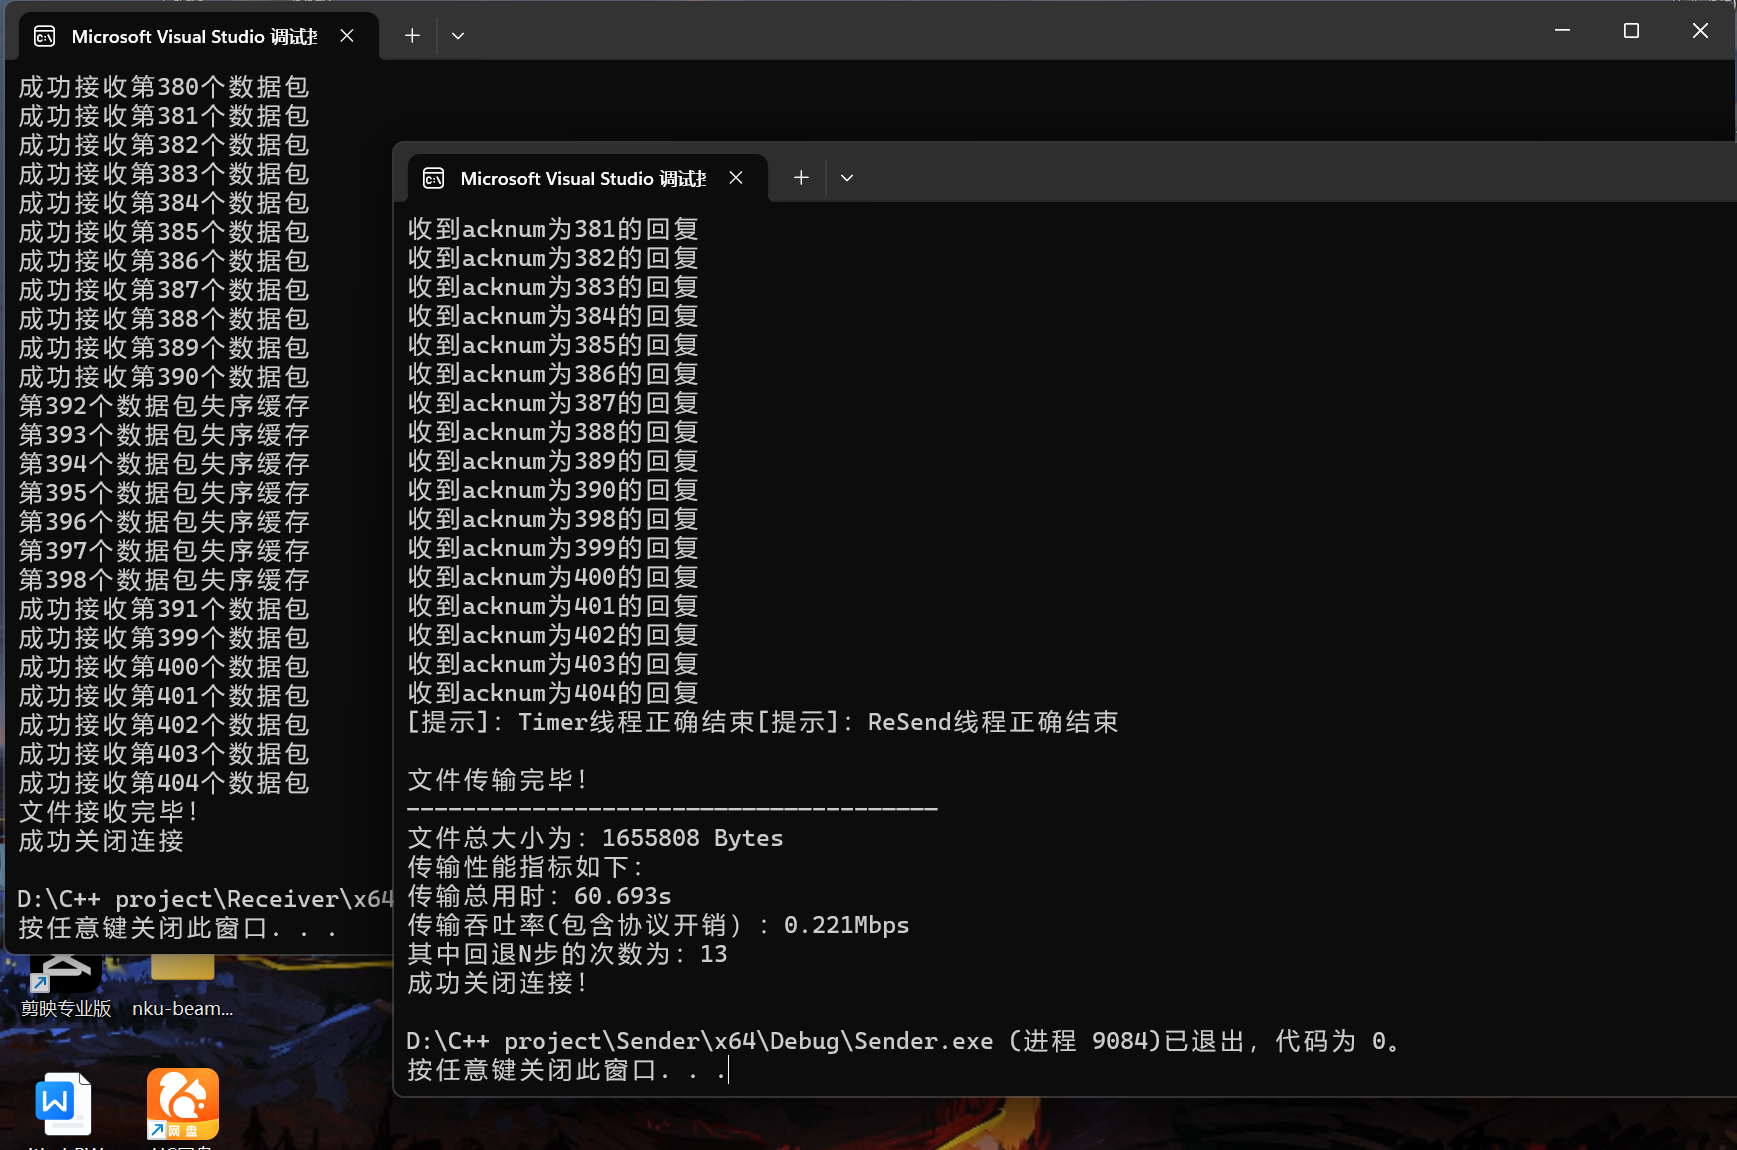
\includegraphics[width=0.8\textwidth]{img/传输helloworld.png}
    \caption{传输helloworld}
\end{figure}
可以看到,程序成功完成了本次传输并且正常关闭连接,在发送端目录下能看到传输的helloworld.txt文件,大小与源文件大小相同。传输1.jpg文件结果如下:
\begin{figure}[H]
    \centering
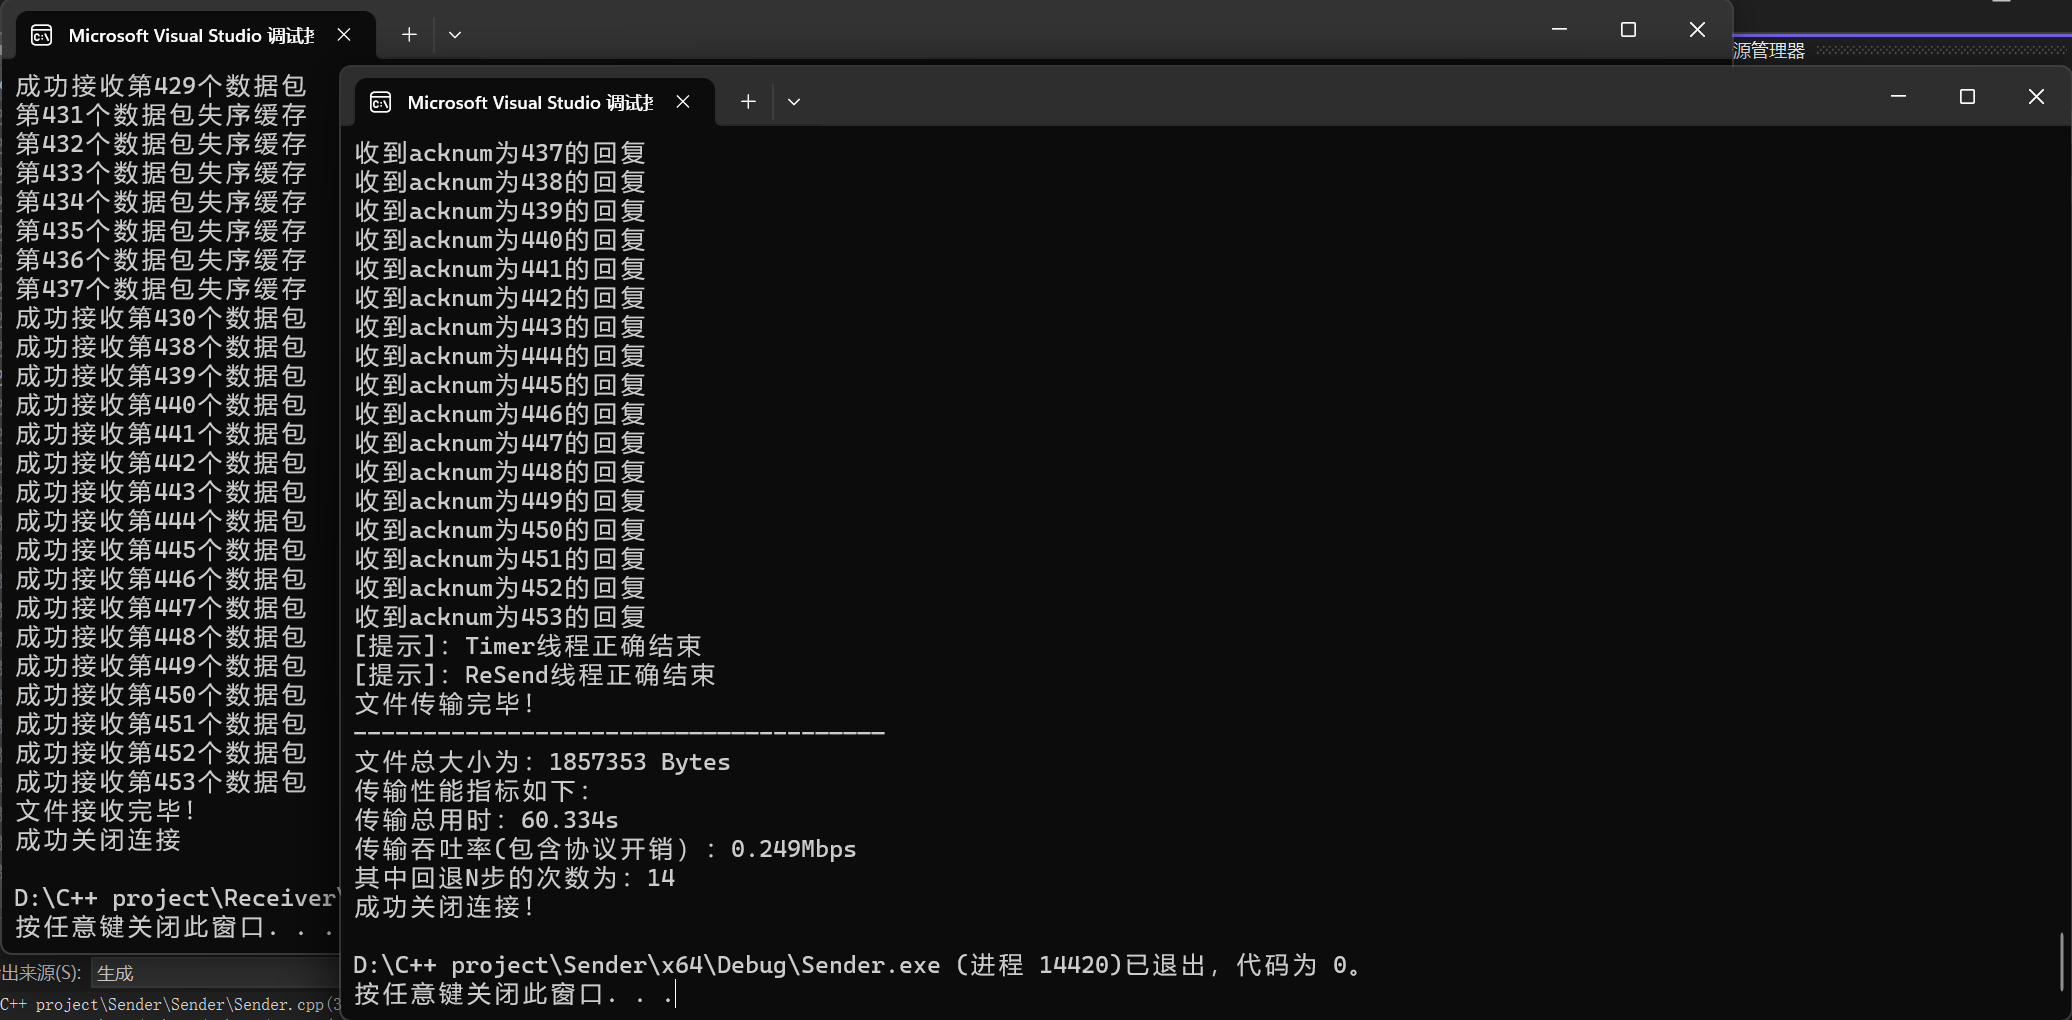
\includegraphics[width=0.8\textwidth]{img/传输图片1.png}
    \caption{传输图片1}
\end{figure}
传输2.jpg文件结果如下:
\begin{figure}[H]
    \centering
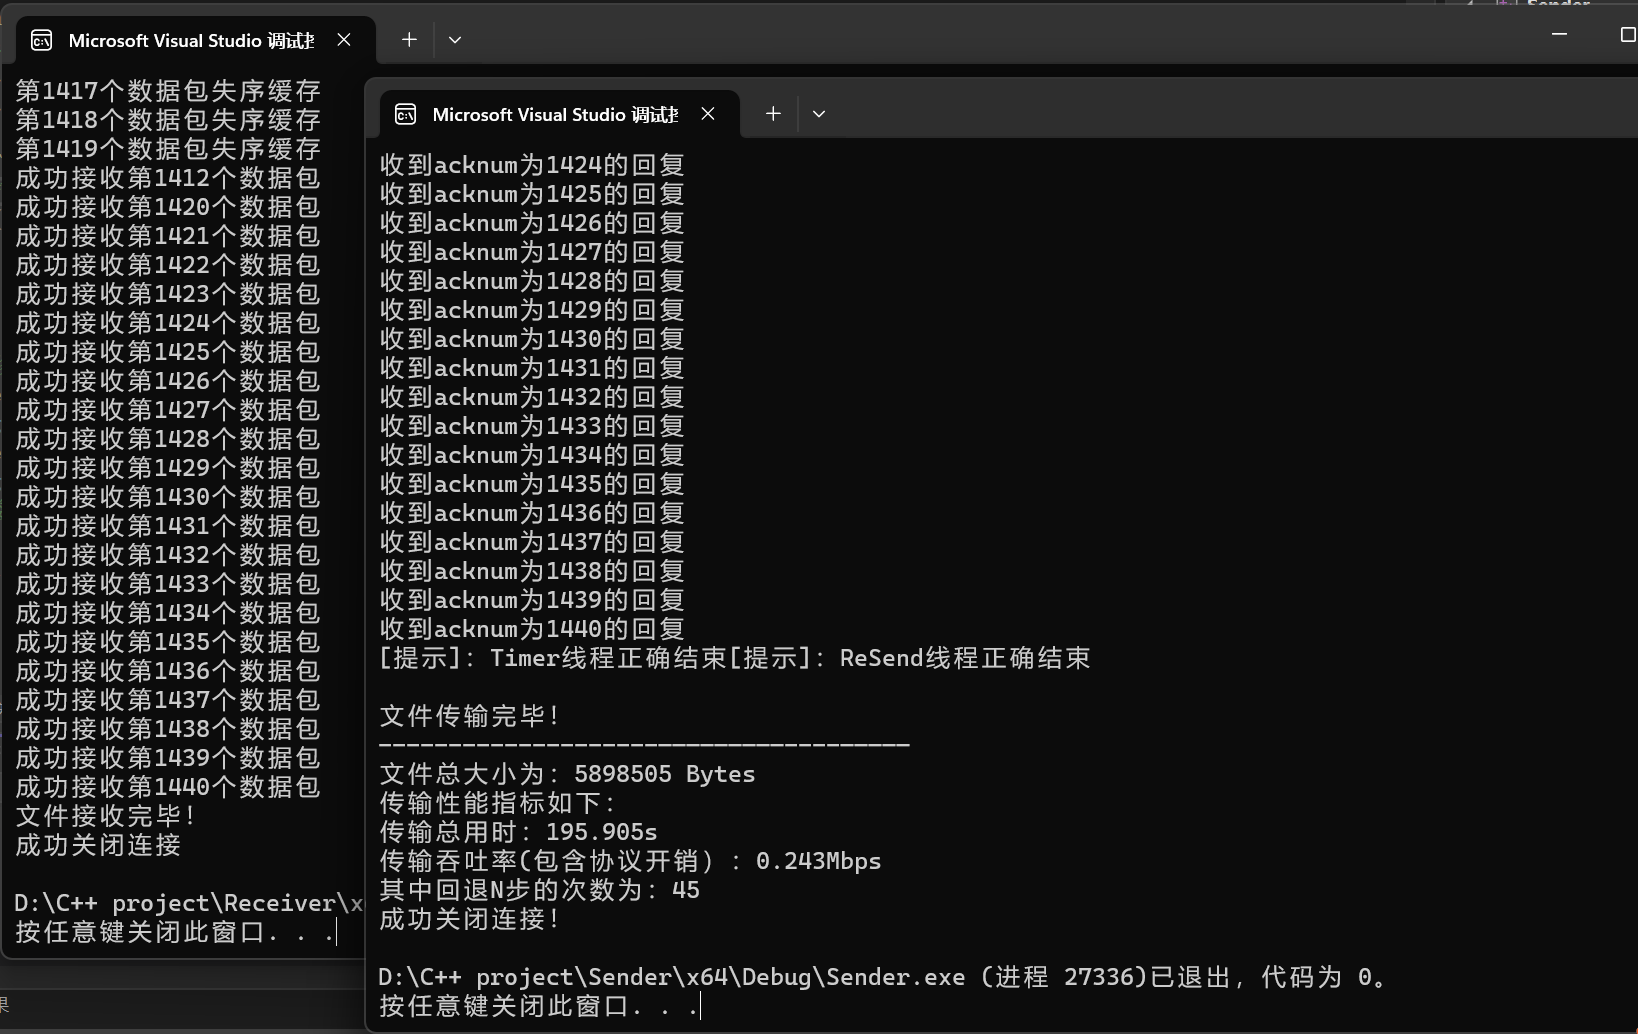
\includegraphics[width=0.8\textwidth]{img/传输图片2.png}
    \caption{传输图片2}
\end{figure}
传输3.jpg文件结果如下:
\begin{figure}[H]
    \centering
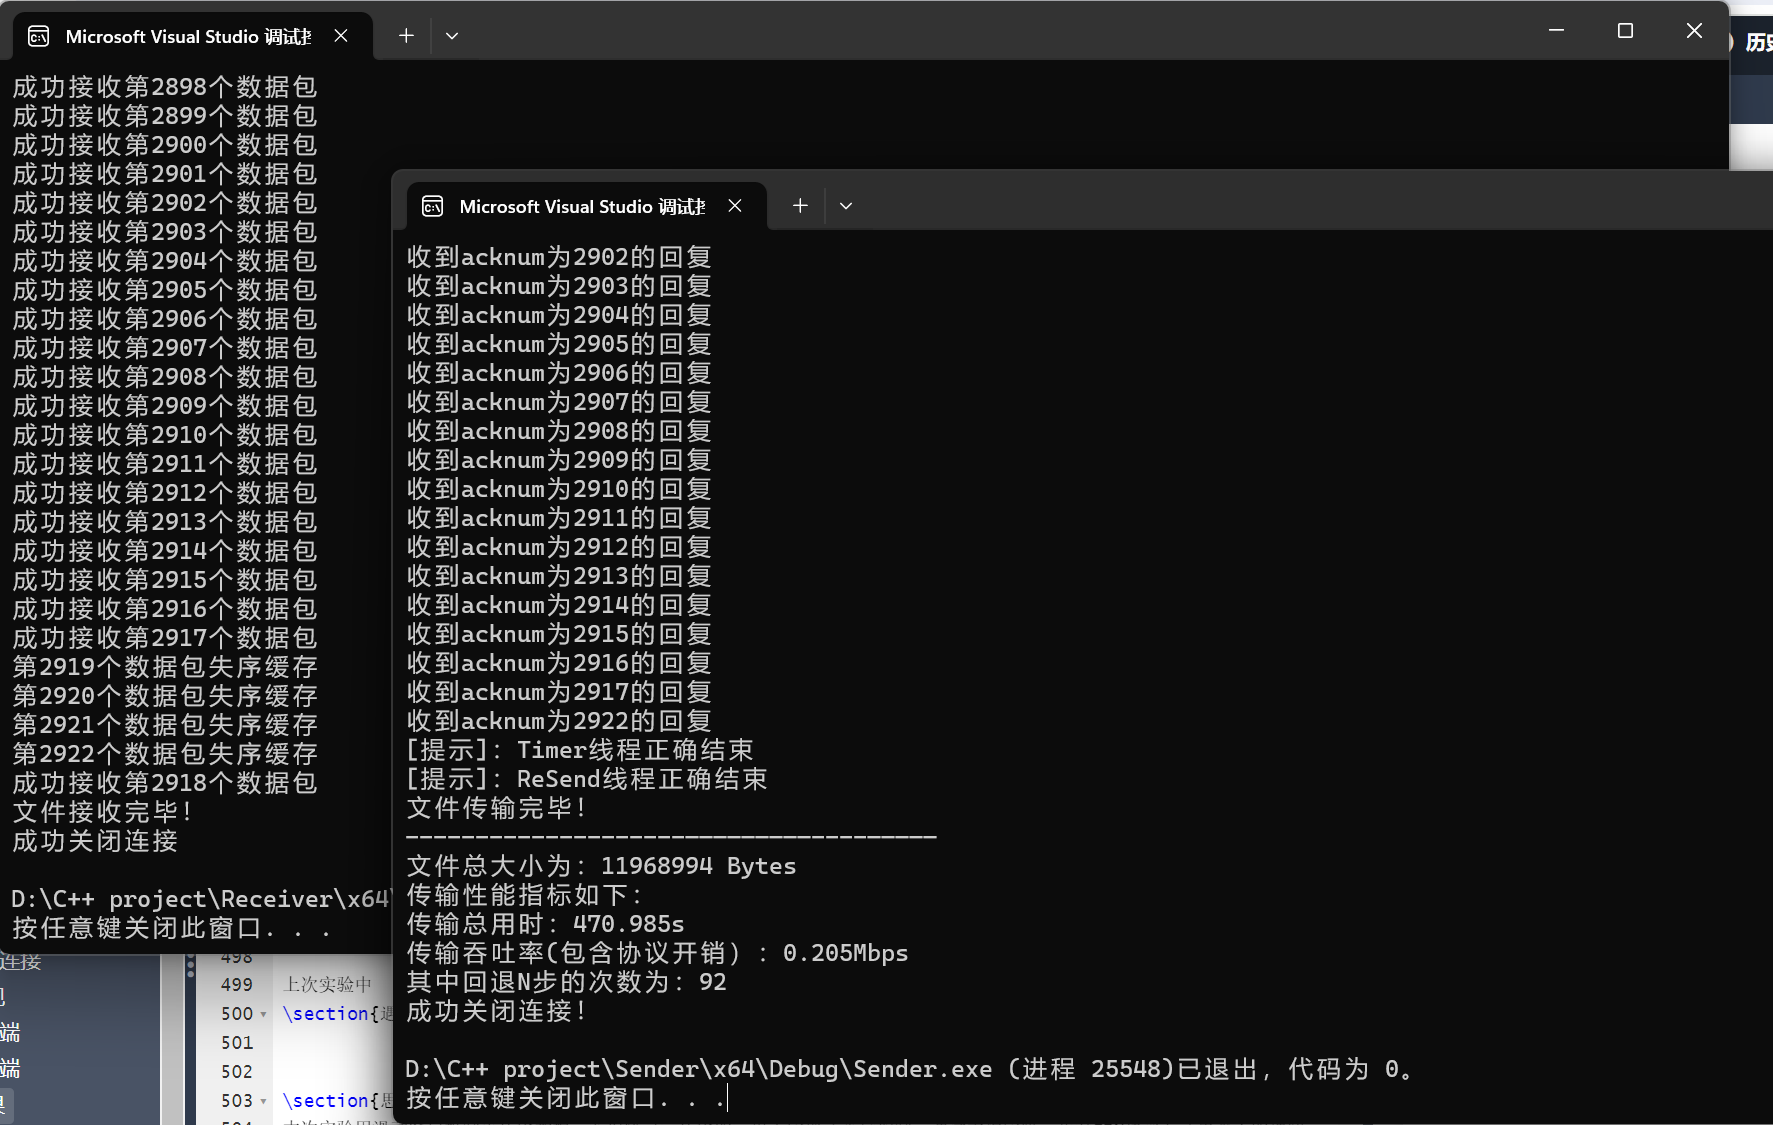
\includegraphics[width=0.8\textwidth]{img/传输图片3.png}
    \caption{传输图片3}
\end{figure}
最后我们分别打开发送端和接收端的 VS 项目文件夹,把传输的四个文件与源文件大小进行比对,发现字节数均相同,说明传输成功。(这里只展示3.jpg文件的字节数)
\begin{figure}[H]
    \centering
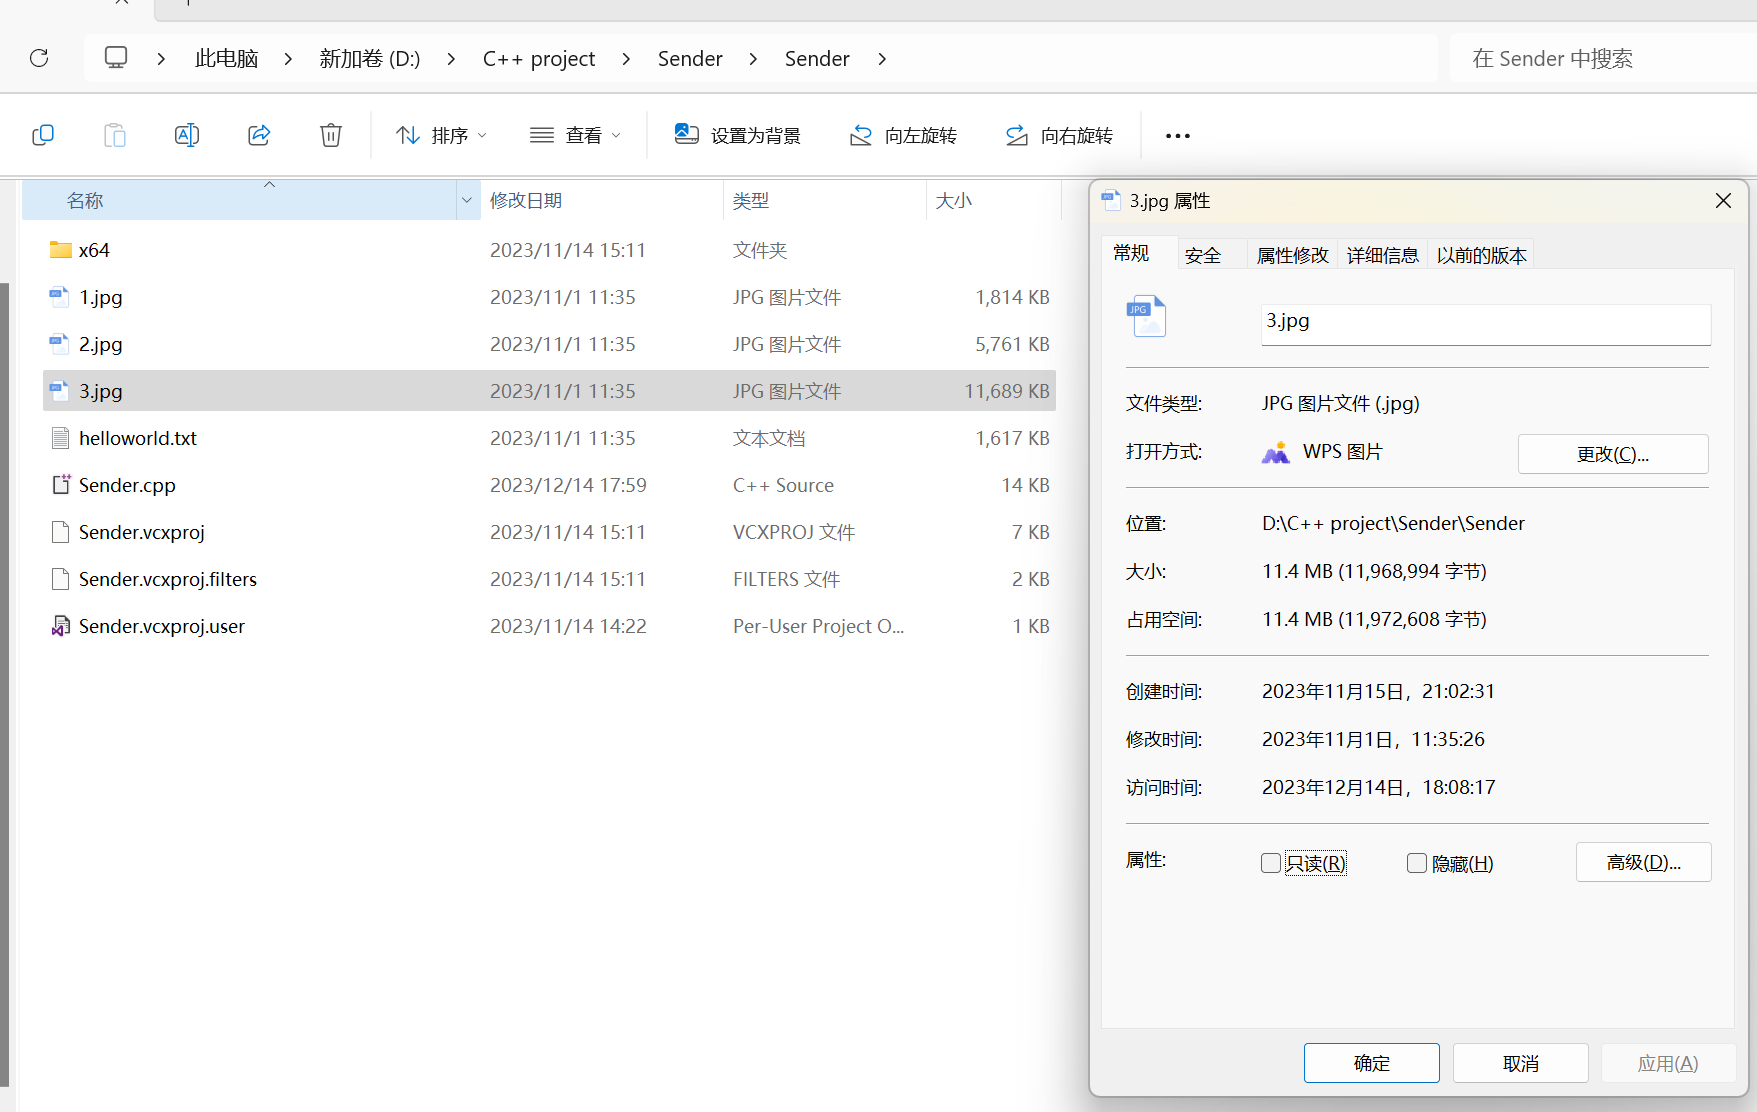
\includegraphics[width=0.8\textwidth]{img/发送端目录.png}
    \caption{发送端目录}
\end{figure}
\begin{figure}[H]
    \centering
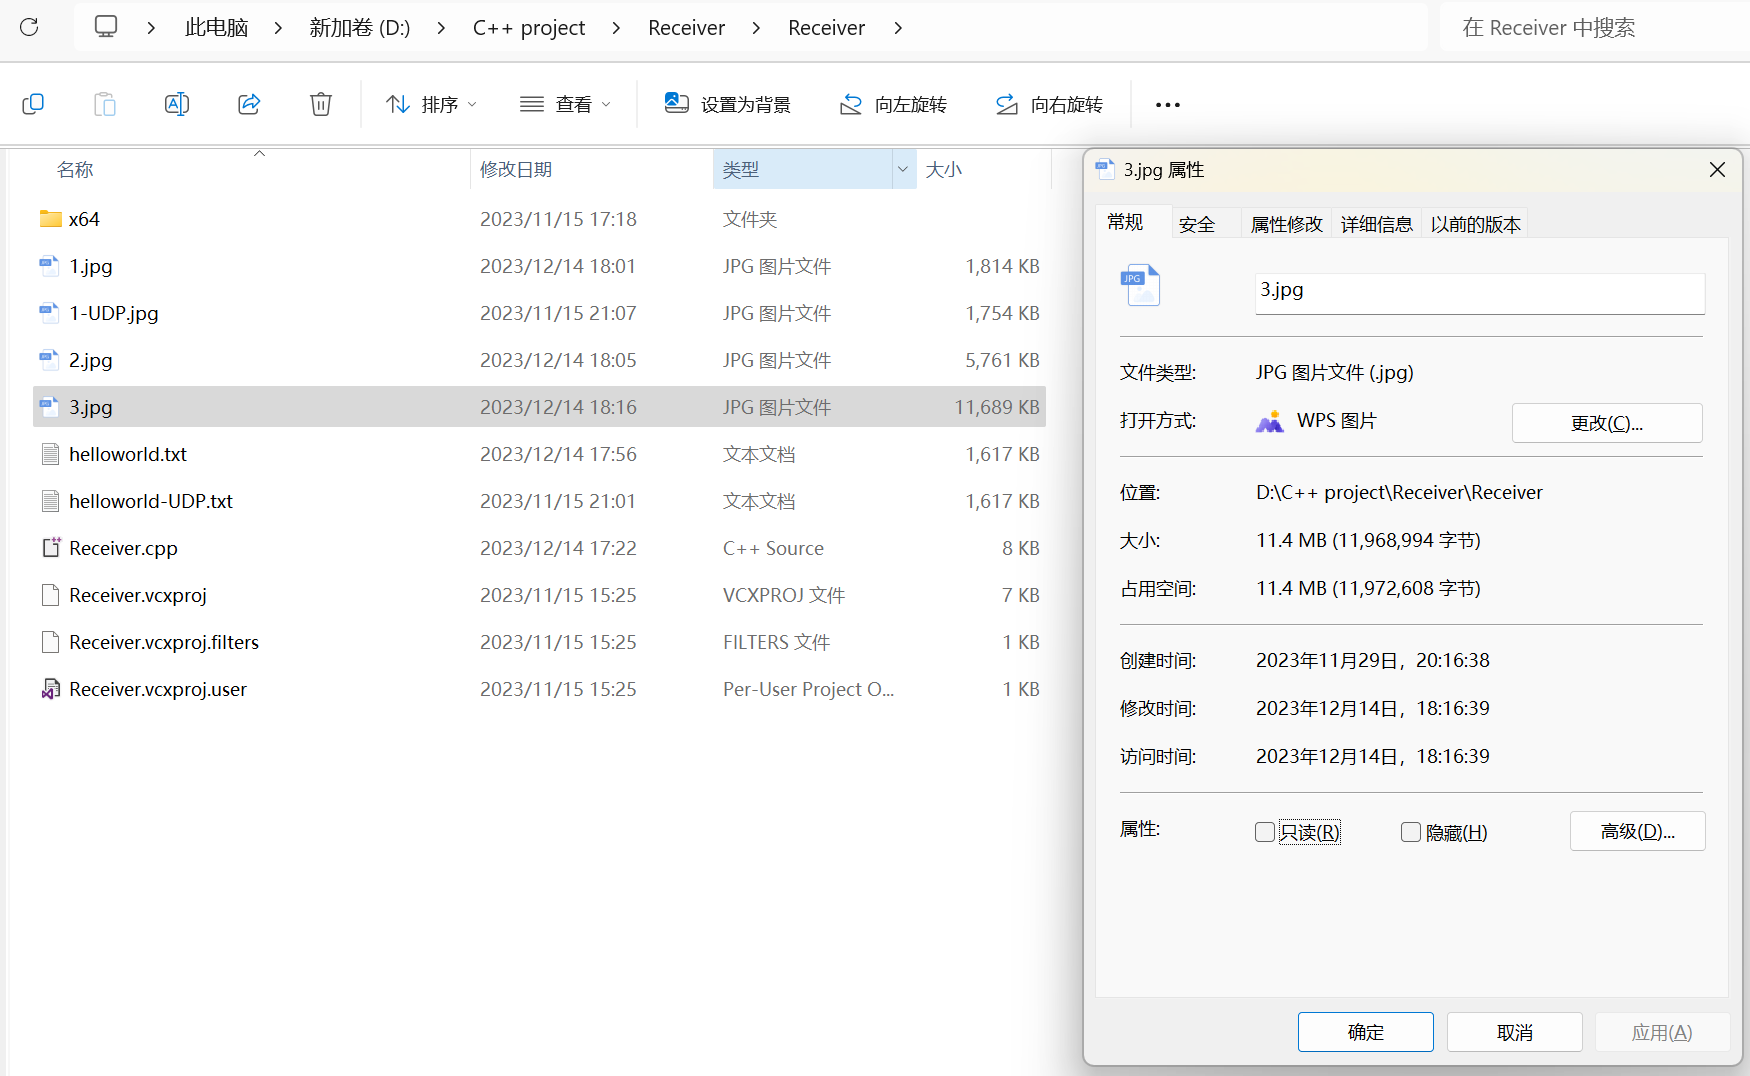
\includegraphics[width=0.8\textwidth]{img/接收端目录.png}
    \caption{接收端目录}
\end{figure}
另外我们发现这四次传输的吞吐率,相较于上一次采用累积确认传输的吞吐率有明显的提升,提升则是在于重传时无需传输整个窗口,在3\%的丢包率情况下,选择确认甚至只需要单独重传丢失的那一个包即可。接下来以传输 helloworld.txt 为例,测试在不同丢包率环境中的传输吞吐率,并用 stata 软件绘制出折线统计图。给定窗口大小为8,超时时间为1.5s,延时为5ms的条件,结果如下(横坐标为丢包率,单位为\%,纵坐标为吞吐率,单位为 Mbps):
\begin{figure}[H]
    \centering
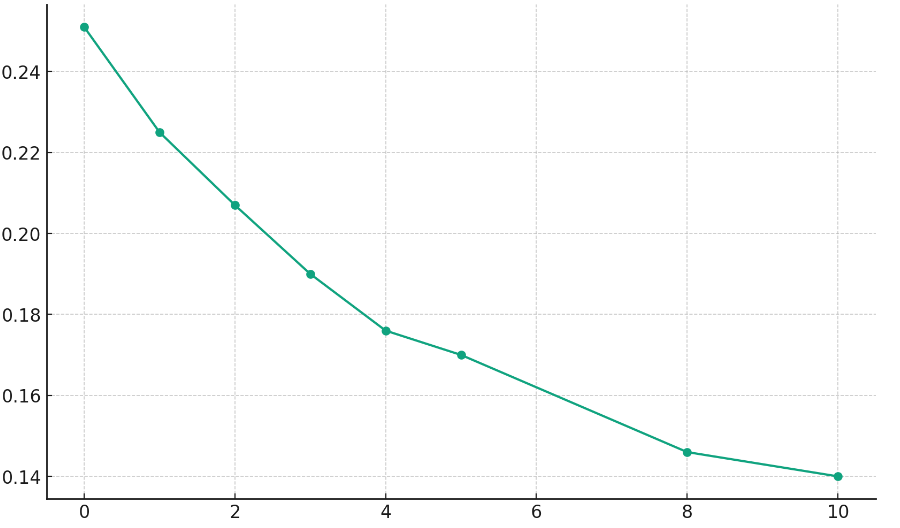
\includegraphics[width=0.8\textwidth]{img/折线图.png}
    \caption{折线图}
\end{figure}


\section{遇到的问题\&解决方法}

Q1: 选择确认需要接收端缓存下失序的数据包,数据包存在哪儿?\par
A: 在之前的实验中,接受端只需要维护一个期望序列号,如果相等则直接写回文件,写回文件的数据包自然有序。而选择确认意味着需要处理失序的数据包,但最后又需要按序交付给文件,这就需要用数据结构来保存数据包,按理说其实可以开一个发送端窗口大小的数据包数组来缓存数据,Expected增加时则把此前的数据包写回文件,但代码实现起来相对复杂。实验中直接开辟了一个大的数据来存所有收到的数据包,传输完毕后最后一次性写回文件即可,缺点是空间开销较大。

\vspace{1cm}

Q2: 接收端怎么告诉发送端哪些数据包已经缓存?\par
A: 本次实验实现选择确认最核心的即是双方的 flag\_cache 数组,接收端在“填补”好缺失的数据包后,需要依据该数组来增加ExpectedNum,从而更新 acknum 并回复报文。在缓存失序数据包的时候,这里的“缓存”其实跟直接存下来是同样的操作,都是直接放回 Buffer 数组中,只不过需要用 sack 报文单独只是哪个包缓存了,这个 sack 和 sacknum 或许可以称作“失序确认”和“失序确认号”,本质上和累积确认号是一个思路,都是通知发送端收到了某一个包,只不过一个是失序,一个是按序。发送端进而可以捕捉到这类型的数据包,并设置 flag 标志位,重传时则利用标志位跳过失序报文。\par

\section{思考与总结}
三次基于 UDP 的可靠传输实验全部结束。通过三次实验,我对网络协议有了一个更深入和更全面的理解和认知。所谓协议,个人把它理解为一种“约定”,一种“标准”,即接收和发送双方共同遵守的规则。协议设计没有问题的情况下,双方都按照规则做事,则数据能够成功传输。但如果一方不遵守约定,传输也会出现错误。比如在实验中,双方实现约定好建立连接的时候,发送方把文件名放入空闲的数据缓冲区。那么接下来则是,发送方按照约定把文件名放进去,接收方按照约定从收到数据包的缓冲区中读取。如果其中有一方不按规则操作,那么最终文件名无法正确传输到接收方手中,这其实就是一种协议。网络这种东西,本质还是一个分布式的系统,没有一个中心化的机构来进行管理,而网络协议则定义了网络中的设备如何相互通信和交换数据,维系着这个互联网的运转。

\end{document}
